\chapter{Einleitung}
\label{chap:einleitung} Die \ac{CT} hat die Medizintechnik revolutioniert und
zählt bis heute zu den wichtigsten Grundlagen der Bildanalyse. Sie stellt eine entscheidende
Weiterentwicklung der klassischen Röntgentechnik dar. Für ihre bahnbrechende
Entwicklung wurden Godfrey Newbold Hounsfield und Allan McLeod Cormack im Jahr
1979 mit dem Nobelpreis für Medizin ausgezeichnet \citep[vgl.][S.~12]{handels2000}.
Dank dieser innovativen Technik lassen sich detaillierte Krankheitsanalysen
durchführen, die eine gezielte und individuell angepasste Behandlung ermöglichen.
Damit trägt die Computertomografie maßgeblich zur Optimierung der medizinischen
Versorgung bei und verbessert die Effektivität therapeutischer Maßnahmen \citep[vgl.][S.~207]{de20083d}.

Die Einsatzmöglichkeiten der Computertomografie sind vielfältig und werden im wahrsten
Sinne des Wortes von Kopf bis Fuß eingesetzt. So kommt es, dass die Computertomografie
auch in der Zahnmedizin eine zentrale Rolle spielt. Die Abbildung
\ref{fig:ct_aufnahme_eines_zahns} zeigt eine solche Aufnahme, wie sie zu Forschungszwecken
eingesetzt wird.

\begin{figure}[h]
	\centering
	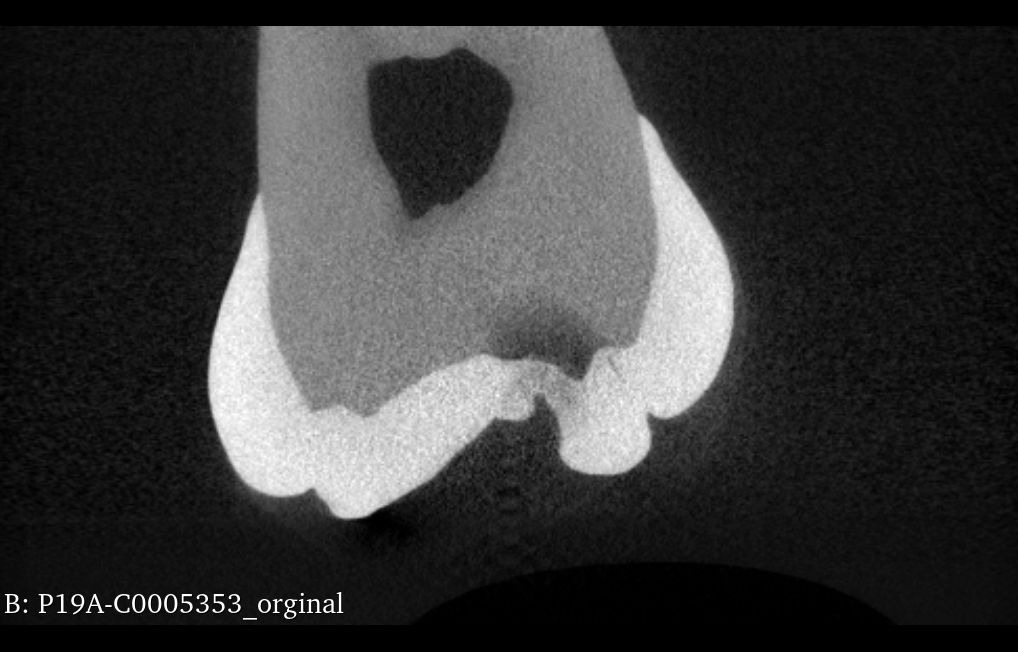
\includegraphics[width=0.5\textwidth]{img/micro_ct_orginal.jpg}
	\caption{CT-Aufnahme einer Zahnkrone nach \citet{heck2024}}
	\label{fig:ct_aufnahme_eines_zahns}
\end{figure}

Mikro-\ac{CT}-Aufnahmen von Zähnen liefern hochauflösende Bilder der inneren Zahnstruktur
und sind damit eine essenzielle Grundlage für die zahnmedizinische Forschung.
Sie ermöglichen nicht nur eine präzisere Diagnostik, sondern auch weiterführende
wissenschaftliche Analysen, beispielsweise zur Untersuchung von Kariesverläufen
oder zur Entwicklung neuer Behandlungsmethoden. Eine konkrete Anwendung zeigt die
Forschung der Poliklinik für Zahnerhaltung und Parodontologie an der \ac{LMU}.
% ---------------------------------------------------------------------------------------

\section{Relevanz der Arbeit}
\label{sec:relevanz_der_arbeit} Damit eine Forschung überhaupt möglich ist, sammelt
die Poliklinik für Zahnerhaltung und Parodontologie Bilddaten in großen Mengen.
Dabei entstehen Aufnahmen der unterschiedlichsten Art, darunter einfache Bilddateien,
Infrarotbilder und insbesondere die für diese Arbeit relevanten
dreidimensionalen Mikro-\ac{CT}-Aufnahmen. Dieser umfangreiche Datenschatz soll
künftig genutzt werden, um ein neuronales Netzwerk zu trainieren, das
statistische Aussagen über das Verhalten von Karies treffen kann \citep[vgl.][S.~1]{walter2025projekt}.
Damit dieses Ziel erreicht werden kann, müssen die Mikro-\ac{CT}-Bilder jedoch
zunächst in eine geeignete Form gebracht werden. Rohdaten allein sind für eine weiterführende
Analyse nur bedingt nutzbar, da sie komplexe Strukturen enthalten, die erst durch
gezielte Verarbeitung sinnvoll interpretiert werden können. Eine der zentralen
Herausforderungen dabei ist die Segmentierung, also die präzise Trennung der verschiedenen
Gewebetypen wie Zahnschmelz und Dentin \citep[vgl.][S.~359]{lehmann2013bildverarbeitung}.
Erst durch diesen Schritt lassen sich anatomisch aussagekräftige Modelle erstellen,
die als Grundlage für Diagnosen, Rekonstruktionen und weiterführende computergestützte
Verfahren dienen. Besonders für das Training neuronaler Netzwerke ist eine
saubere Segmentierung essenziell, da sie die Qualität und Aussagekraft der daraus
gewonnenen Erkenntnisse maßgeblich beeinflusst. Dadurch lässt sich
beispielsweise auch der \textit{Ground Truth} für ein neuronales Netzwerk verbessern,
da die Kariesklassifizierung mit segmentierten Daten deutlich einfacher ist.
% ---------------------------------------------------------------------------------------

\section{Ziel der Arbeit}
\label{sec:ziel_der_arbeit} Das Erzeugen von segmentierter Daten aus einem Mikro-\ac{CT}
ist jedoch nicht trivial und verlangt komplexe Techniken der \ac{3D}-Bildbearbeitung.
Der aktuelle Stand der Kunst zeigt, dass es bereits ein Verfahren gibt, mit dem solche
Daten erzeugt werden können. Hierbei unterteilt das Verfahren ein gegebenes
Mikro-\ac{CT}-Bild in die zwei Gewebesubstanzen Dentin und Schmelz. Dieser
Vorgang kann als anatomische Segmentierung des Zahns bezeichnet werden. Die Ergebnisse
des Verfahrens sind vielversprechend. Jedoch bringt es auch einige Limitierungen
mit, was die Benutzung deutlich einschränkt. Eine dieser Limitierungen bezieht
sich auf die Art der Ausführung. Zum aktuellen Stand muss das Verfahren aufwendig
über ein Terminal gestartet werden. Dies stellt für praktizierende Ärzte, die letzten
Endes die Anwendergruppe dieses Verfahrens sind, eine besondere Herausforderung
dar.

Die vorliegende Arbeit widmet sich genau dieser aktuellen Herausforderung. Ziel ist
es, eine Benutzerschnittstelle zu entwickeln, die den Anwender mit der anatomischen
Segmentierung verbindet und so die Verwendung des Verfahrens deutlich vereinfacht.
Darüber hinaus soll eine Struktur geschaffen werden, mit der es möglich ist,
Mikro-\ac{CT}-Bilder effizient und interaktiv über eine Benutzerschnittstelle zu
Betreiben, ohne das dabei Einschränkungen in Bezug auf die Qualität gemacht
werden müssen. Da Mikro-\ac{CT}-Bilder weltweit eine zentrale Rolle in der
zahnmedizinischen Forschung spielt, bietet sich für eine interaktive Nutzung die
Plattform 3D Slicer an. Diese etablierte Software wird in zahlreichen Kliniken
und Forschungseinrichtungen weltweit zur Verarbeitung und Analyse medizinischer
Bilddaten eingesetzt. Aufbauend auf dieser Grundlage soll nun eine spezielle Benutzerschnittstelle
innerhalb 3D Slicer entwickelt werden, die auf der vorhandenen Modul- und Plug-in-Infrastruktur
der Plattform basiert. Diese Infrastruktur bietet die Möglichkeit, eigene Module
mit individuellen Algorithmen zu befüllen, eine Schnittstelle bereitzustellen
und diese nahtlos in das Kernsystem zu integrieren. 3D Slicer sieht hierfür die Implementierung
einer \ac{SEM} vor. Hierbei handelt es sich um einer Erweiterung oder ein Plug-in
für die 3D Slicer Kernanwendung. Durch die Bereitstellung von segmentierten
Daten in einer \ac{SEM} würde so nicht nur die der aktuellen Forschungsumgebung einen
Mehrwert erhalten, sondern die gesamte Zahnmedizin.

Bei der Umsetzung dieser Erweiterung stehen nicht nur die funktionalen
Anforderungen im Fokus, sondern auch softwaretechnische Qualitätskriterien. Eine
möglichst generische Architektur soll gewährleisten, dass das Modul flexibel bleibt
und künftig um weitere Funktionalitäten erweitert werden kann.

Mit diesen konkreten Zielsetzungen lässt sich nun eine Forschungsfrage ableiten,
die in dieser Arbeit im Fokus stehen soll.

\begin{center}
	\textit{Wie kann eine benutzerfreundliche Schnittstelle innerhalb von 3D
	Slicer entwickelt werden, die nicht nur das Verfahren der anatomischen Segmentierung
	effizient integriert und den Zugang für Anwender vereinfacht, sondern auch
	eine strukturierte und flexible Umgebung zur Verarbeitung von Mikro-\ac{CT}-Aufnahmen
	bietet?}
\end{center}

Um das in dieser Arbeit zu entwickelnde Modul optimal in den bestehenden Prozess
der anatomischen Segmentierung zu integrieren, ist es essenziell, zunächst ein grundlegendes
Verständnis dieses Verfahrens zu erlangen. Daher wird im folgenden Kapitel
erläutert, wie die anatomische Segmentierung funktioniert, welche Techniken und
Algorithmen dabei zum Einsatz kommen und welche Herausforderungen sich daraus
ergeben. Dieses theoretische Fundament bildet so die Basis für die darauf aufbauende
Entwicklung einer 3D Slicer Erweiterung.
% ---------------------------------------------------------------------------------------